\lettrine[lines=2]{\color{BrickRed}H}{aving} outlined key concepts and methodology, and after literature studies were collected, inspected and coded using general inductive approach, this chapter constructs and formalizes ten data science design patterns. 
It then establishes \acl{DSTM} too.

%%%%%%%%%%%%%%%%%%%% 
\section{Pattern 1: Notebook}

\paragraph*{Context}
An iterative, interdisciplinary \ac{DS} process, as illustratively seen on the \ac{CRISP-DM} methodology and Figure \ref{fig6}, consists of many different phases that are accomplished during a life-cycle of an analytical project.

\paragraph*{Problem}
To enable easier communication with stakeholders in the course of insights discovery from data large and small, it is necessary to document approaches to questions being asked and manage acquired knowledge in a systematic way.

\paragraph*{Forces}
\begin{compactitem}
   \item \ac{DS} is an incremental procedure where exploratory analysis needs to be explicitly described alongside the information such as what are the business objectives to solve, who are the stakeholders involved, where do data come from and how are they treated.
   \item Being related to the software engineering, the aim is to stay within a workflow of the centralized repository for source code management.
   Thus, the document should be stored in an open format enabling tracking of changes in it by means of a version control system like \mintinline{bash}/Git/.
\end{compactitem}

\paragraph*{Solution}
Initially, \ac{KDD} process may start from \ac{DS} \emph{notebooks} which support a lightweight markup language such as Markdown used to chronicle the progress and that in addition are accompanied by specifically marked code snippets. 
Upon running this master file, results are printed in line with the other text rendered too.
In short, it combines source code with readable description that is capable of recording not only small comments but also \ac{DS} project plan with gathered information from the stakeholders. 
At the same time, \emph{notebooks} present data analysis in a visual and concise form as well \parencites{WilsonGred2017}{NatureBPDASNMRI2017}. 

\paragraph*{Consequences} ~\\
{\hspace*{14.5pt} \textbf{Benefits:} \hspace*{-5.5pt} }
Sharing \emph{notebooks} simplifies reproducibility due to publishing the source code with graphics \parencite{JakeVanderPlas2016PythonHandbook}.
Likewise, by transparently communicating research activities that lead to achieved outcomes, they enhance organizational collaboration and memory through careful document management \parencites{JonJupyter2016}{CharlerSutton2012}.
Moreover, they permit fast collection of the feedback from the \ac{DS} team by executing individually \emph{notebook's} code examples, thus promoting lean and interactive development style \parencites{EslamiAli2012}{CMACanada2003}.

\textbf{Liability:}
Being split into smaller code chunks instead of stored in cohesive files, source code becomes hard to orient in.
Because of a tendency of having code snippets across multiple \emph{notebooks} (\enquote{here and there}), it creates a need for following a priori and well-defined structure with appropriate naming conventions for data, files and folders to minimize plausible disorganization \parencite{FieldCadyDSBook}.

\paragraph*{Known uses}
\begin{compactitem}
   \item \emph{Notebooks} encourage quick prototyping and iteration on modelling and processing steps for the data analysis, see later \patternName{Prototyping Design Pattern}. 
   \item Because of richness of supported presentation formats, they are used for storytelling of insights through an explanation of chosen approaches, conducted tasks and a discussion of actionable results.
   \item Additionally, authors like \textcite{JakeVanderPlas2016PythonHandbook} utilize these to write tutorials, data dictionaries, technical reports and even books teaching computer science concepts or programming languages.
\end{compactitem}

\paragraph*{Related Patterns}
\emph{Notebooks} can contain embedded interactive visualizations which enable users to interplay for instance with check boxes or sliders, see \patternName{Interactive Application Design Pattern}.

Not having \ac{DS} project including \emph{notebooks} checked into the previously mentioned version control systems such as \mintinline{bash}/Git/ that supplement recording of a \emph{project history} culminates into lacking a holistic view of its past development and ability of restoring changes by going back in time. 

\paragraph*{Sample Code}
Practitioners and researchers can choose between \mintinline{R}/RMarkdown/ package (typically in conjunction with RStudio \ac{IDE}) and \mintinline{python}/Jupyter/, a browser-based application. 
Both tools provide functionality for keeping a \ac{DS} journal and support many different output formats including \ac{HTML}. 
Similarly, they are programming language independent whereby R, Python, Ruby and Haskell could all be used within the same file. 

To organize the R and Python source code and simplify its reproducibility, where appropriate, all snippets in \textbf{this chapter} are presented by means of either instrument, see Figure \ref{lst:code_pattern1}.

\begin{figure}[!ht]
\centering
\includegraphics[width=\textwidth, height=8cm, keepaspectratio]{images_dp/code_listing_1_notebook}
\caption[Example for Notebook Design Pattern.]{The example for \patternName{Notebook Design Pattern} shows R Markdown file (\path{code_data/R_masterThesis.Rmd}) consisting of R snippet alongside the comments. 
When this file is executed, \ac{HTML} page is rendered, part of which can be seen in Figure \ref{lst:code_pattern2} of the next design pattern.
The alternative utilizing \mintinline{python}/Jupyter/ can be found in \path{code_data/Py_masterThesis.ipynb}.}
\label{lst:code_pattern1}
\end{figure}

%%%%%%%%%%%%%%%%%%%%%%%%%%%%%%
\section{Pattern 2: Data Frame}

\paragraph*{Context}
After stakeholders asking a set of questions that have a direct impact on company's sales, hypotheses together with an unambiguous project plan and well-defined objectives and scope are developed. 
Next, right data sources are identified which is finally followed by their acquisition.

\paragraph*{Problem}
When using programming languages like R and Python, data scientists need to programmatically manipulate and query two-dimensional data by applying one common interface.

\paragraph*{Forces}
\begin{compactitem}
   \item Data are stored in a variety of locations and formats which encumbers any further combined operations on them.
   \item Providing wisdom about business operations by storing high-quality internal and external data in the centralized \ac{DW} (Figure \ref{fig-bi-dw-schema}) is significantly limited by the available \ac{SQL} functions which usually do not contain advanced statistical methods, thereby prohibiting their analysis.
   \item These days, however, there is a need for flexible application of research's latest and cutting edge algorithms that are typically not immediately accessible even in the conventional \ac{BI} portals, \ac{ETL} and visualization tools.
\end{compactitem}

\paragraph*{Solution}
Another fundamental principle on which \ac{DS} depends are \emph{data frames}. 
These abstract and most commonly in-memory data structures allow engineers to store and process various types of raw information in a unifying fashion and without a reliance on other third-party applications, mainly the database management systems. 
Being in a tabular form, \emph{data frames} consist of rows representing observations and which might be heterogeneous and columns describing variables with labels (these should be as a whole homogeneous; \cite{Mikut2011}). 

\paragraph*{Consequences} ~\\
{\hspace*{14.5pt} \textbf{Benefits:} \hspace*{-5.5pt} }
Taking an inspiration from the data warehousing, \emph{data frames} can be sliced and diced using operations such as \mintinline{R}/subset()/ or \mintinline{R}/aggregate()/ for further data manipulation, including their visualization \parencite{DWSlideDice}. 
Besides treating missing data in a consistent matter, they can be also serialized into binary files, and thus easing the reproducibility and sharing of the results \parencite{JakeVanderPlas2016PythonHandbook}. 

\textbf{Liability:}
Storing a condensed \emph{data frame} is significantly restricted by the available \ac{RAM}, and therefore persistence of data, its velocity and volume being important properties have to be considered in advance \parencites{SimonBGDRAMR2016}{Fern2016}. 
Additionally, because data structures vary by underlying implementations, any performance tuning and exposed operations and syntax through \ac{API}, it brings a gradual learning curve to known them thoroughly when working with multiple languages and tools offering similar functionality.

\paragraph*{Known Uses}
\begin{compactitem}
   \item A typical use case scenario is extracting and loading data for example from databases or spreadsheet files, see \textcites{NinaBookR2014}{PSDS2017}.
   \item Principally, being essential in the end-to-end \ac{KDD} process, \emph{data frames} are used at all \ac{DS} stages for steps that include pre-processing, merging data with other datasets and transforming them for exploratory analysis and statistical modelling.
\end{compactitem}

\paragraph*{Related patterns}
\emph{Data Matrix} is another two-dimensional data structure on top of which \emph{data frames} are build.
Yet, its implementation details differ in the R and Python universe. 
While R's natively offered \mintinline{R}/matrix()/ as well as \mintinline{R}/Matrix()/ from \mintinline{R}/Matrix/ package can only consist of data of the same type, for example only integers, \mintinline{python}/matrix()/ implemented in Python's \mintinline{python}/NumPy/ package may hold data of different types too \parencites{Numpy2011}{MatrixCran2017}. 
Therefore, being more like \emph{data frames}.

\paragraph*{Sample code}
Two R (\mintinline{R}/tibble/ and \mintinline{R}/data.table/) and Python (\mintinline{python}/pandas/ and \mintinline{python}/blaze/) packages were identified providing a mechanism to store data in a tabular format, see Figure \ref{lst:code_pattern2}.  

\begin{figure}[!ht]
\centering
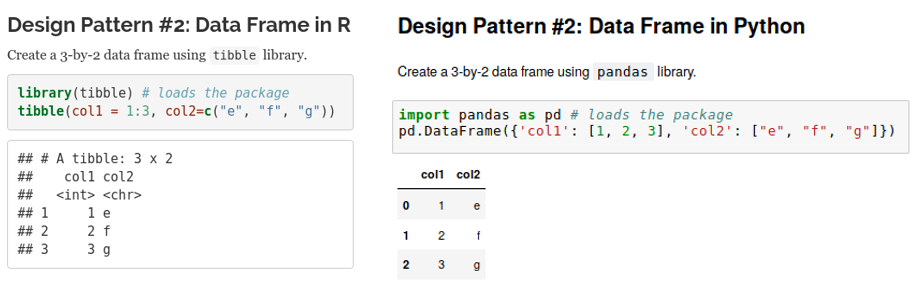
\includegraphics[width=\textwidth+2cm,height=\textheight,keepaspectratio]{images_dp/code_listing_2_df}
\caption[Example for Data Frame Design Pattern.]{The example for \patternName{Data Frame Design Pattern} demonstrates two \emph{data frames} being created. 
While on the left \mintinline{R}/tibble/ is displayed when rendering the previous Figure \ref{lst:code_pattern1}, on the right Python's \mintinline{python}/pandas/ is shown.
The source code for this pattern is located in \path{code_data/R_masterThesis.Rmd} file, \path{code_data/Py_masterThesis.ipynb} respectively.}
\label{lst:code_pattern2}
\end{figure}

%%%%%%%%%%%%%%%%%%%%%%%%%%%%%
\section{Pattern 3: Tidy Data}

\paragraph*{Context}
While \ac{DW} may already store high-quality, rectangular tables in an easy to work with structure, externally captured information is organized in a variety of formats and diverse in their shapes.
After importing it from different \ac{IT} systems and web services, data frames are formatted to facilitate knowledge discovery.
Although processing has been argued to take the largest effort, depending on studies anywhere between 30\% and 80\%, the accurate and clean data stored in a right way make it simple to handle any \ac{DS} task \parencites{ThomasZeutschler2016ITAnalytics}{Taft2015}.

\paragraph*{Problem}
Most typically encountered are messy data which are usually organized in a \emph{wide} format where a table contains one observation (row) across many different variables (columns) for each subject that can be for example a person or a country \parencite{Boehmke2016DataR}. 
Hence, they need to be efficiently changed to become ready for the subsequent analytical investigation. 

\paragraph*{Forces}
\begin{compactitem}
  \item Modifying (big) data by hand may not be accomplished due to their sheer size, complexity and significant time effort leading to potentially introducing errors and having a non-agile \ac{DS} by being distracted from deriving the actionable business results.
  \item At the same time, different \ac{KDD} steps, methods and tools expect one exact arrangement of data forcing professionals to reshape them frequently in the journey through the data pyramid. 
  \item Working with data that may contain several variables \qcite{in one column} or \qcite{in both rows and columns} affects the inquiry on account of having difficulties in their understanding as well as conducting any exploratory operations \parencite[5]{TidyDataWickham2014}.
\end{compactitem}

\paragraph*{Solution}
Spearheaded by \textcite[5]{TidyDataWickham2014}, the concept of \emph{tidy data} has been suggested to \qcite{provide a standard way of structuring a dataset}.
Modelled after \citeauthor{Codd:1970:RMD:362384.362685}'s (\citeyear{Codd:1970:RMD:362384.362685}) third normal form, three core principles were specified, namely (a) each variable forming a column, (b) each observation forming a row and (c) each type of observational unit forming a final table.
As such, this manifests into the \emph{long} data structure where a table spans each subject over multiple observations because of having a column (a key) with variable types such as land area or a population and another one for their corresponding values. 
Being a part of a broader data management where metadata, data stewardship and security are of an importance, the technique of tidying the dataset into a particular layout has become a design convention for organizing analysis-friendly information \parencites{WilsonGred2017}{CMACanada2003}{DataBoK2017}. 

\paragraph*{Consequences} ~\\
{\hspace*{14.5pt} \textbf{Benefits:} \hspace*{-5.5pt} }
Having data in the \emph{long} format simplifies their manipulation and further transformation including filtering or ordering \parencite{NinaBookR2014}.
In this matter, \emph{tidy data} increase users' overall experience by leveraging a consistent approach in coding style due to a potential availability of closely related tools that make the analysis flow easily together, for instance with a sequencing \enquote{\%>\%} pipe operator \parencites{Boehmke2016DataR}{GarrettGrolemund2017RData}.

\textbf{Liability:}
Contrarily, \emph{wide} data might be more straightforward to enter and inspect as they can have column names as values like \enquote{day1} or in ranges such as \enquote{\$10-20k} \parencites{WilsonGred2017}.
Moreover, albeit language neutral, the concept is largely R centric where it stipulates a domain-specific language, a \qcite{sub-dialect of the R} called \emph{tidyverse} -- thus plausibly not directly replicable to other languages \parencite{Rickert2017}. 

\paragraph*{Known Uses}
\begin{compactitem}
  \item Principally, the evidence stored in the \emph{long} style is most frequently imperative for the modelling and visualization purposes and corresponding packages that enable it, see \patternName{Prototyping} and \patternName{Interactive Application Design Pattern} \parencite{TidyDataWickham2014}. 
  \item Within the R's \emph{tidyverse} sub-ecosystem, data in the corresponding shape play an integral role as they work hand in hand with complementary tools, including the previously mentioned \mintinline{r}/tibble/ \parencite{GarrettGrolemund2017RData}.
\end{compactitem}

\paragraph*{Sample code}
For R, a variety of options exist that provide operations for \emph{tidy data}.
When data frames are build using \mintinline{R}/data.table/, it also offers \mintinline{R}/melt()/ and \mintinline{R}/dcast()/ functions for their reshaping which are claimed to outperform the identically titled ones from the original \mintinline{R}/reshape2/ package \parencite{DataTable2017}.
Additionally, within the tidyverse ecosystem, a dedicated application has been developed named \mintinline{R}/tidyr/ too, see its use in Figure \ref{lst:code_pattern4}.

On the contrary, the previously mentioned \mintinline{python}/pandas/ is indispensable in the Python's \ac{DS} ecosystem due to being comprehensive in capabilities it provides, including for data transformation.
Nonetheless, when data are in a more traditional shape of an array or a matrix, \mintinline{python}/NumPy/ library, being a part of the \emph{SciPy} sub-ecosystem, offers its own methods as well.

\begin{figure}[!ht]
\centering
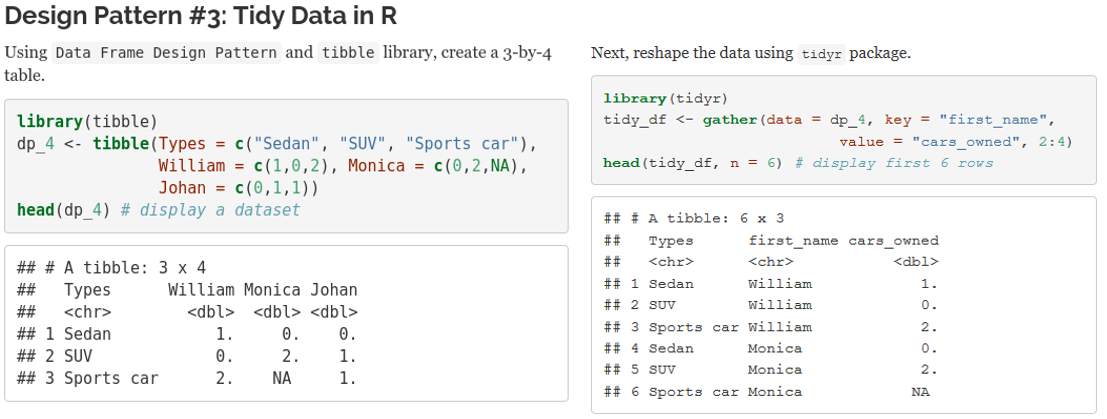
\includegraphics[width=\textwidth+2cm,height=\textheight,keepaspectratio]{images_dp/code_listing_3_td_R}
\caption[Example for Tidy Data Design Pattern.]{An example for \patternName{Tidy Data Design Pattern} shows how a data frame is created using R' \mintinline{R}/tibble/ and subsequently transformed from a \emph{wide} (messy) to a \emph{long} (tidy) format. 
The source code for this pattern is located in \path{code_data/R_masterThesis.Rmd} file, \path{code_data/Py_masterThesis.ipynb} respectively.}
\label{lst:code_pattern4}
\end{figure}

%%%%%%%%%%%%%%%%%%%%%%%%%%%%%%
\section{Pattern 4: Leakage}

\paragraph*{Context}
After data cleaning and formatting, it is still rare that data sets are complete allowing the analysis and modelling to proceed further and make valid conclusions to stakeholders reflecting the stated objectives.
Indeed, when some information is missing or not being in the right quality and quantity, among some not always available and preferred options, it can be crowdsourced from users or be acquired from third-party providers \parencites{Domino2017DS}.

\paragraph*{Problem}
Before \ac{ML} prototypes are created, data scientist need to solve table's missing data as their occurrence is undesirable for many algorithms which often simply omit potentially valuable observations with some lacking values. 
Therefore, the analysis of incomplete facts might be misleading and absent data need to be predicted or otherwise \enquote{imputed}.

\paragraph*{Forces}
\begin{compactitem}
  \item Dropping rows or columns which contain missing values is universally not advisable as it reduces a sample size and introduces a bias to parameter estimates like correlation or standard error \parencite{Gelman2007}. 
  \item At the same time, replacing missingness with median, mode or mean can lead to biased estimates too due to outliers, not considering relationships between features and general uncertainty about the outcomes that is not reflected in the imputed data \parencite{Rubin2002}.
  \item The other so-called \emph{single imputation method} may involve regression where missing values are predicted from complete observations using a regression model. 
  Though, as described by \textcites[6]{ZhangSingleImput2016}{GarcijaGomez2010}, the \qcite{variability of missing values is underestimated} by this approach as only a single regression curve is created. 
\end{compactitem}

\paragraph*{Solution}
In order for data scientists to appropriately handle missing data, one needs to answer an integral question, namely why are they missing.  
According to \textcite[3]{DabneyAlanNormalization2012} three missing data mechanisms are distinguished and consequently the approach to a treatment \qcite{should ideally rely on the mechanism that caused the values to be missing} in the first place. 

\textcite{Rubin2002} have talked about a concept named \emph{missing at random (MAR)} where missing data ($Y_{mis}$) are related to those observed ($Y_{obs}$) and can be predicted from them.
A special case of MAR is when the nature of missing data is not related to input variables -- then data are said to be \emph{missing completely at random (MCAR)}.
This usually happens when the equipment malfunctions or there is an error in data entry -- thus $Y_{mis}$ is neither related to $Y_{obs}$ nor to $Y_{mis}$. 
Both cases are said to be \emph{ignorable} because the reasons for missingness are ignored and \qcite{it is appropriate to impute} such data \parencites[340]{Lynn2002}.
At last, a \emph{nonignorable} situation named \emph{missing not at random (MNAR)} means that the probability of missingness depends on the missing variable itself, for example when a \qcite{sensor cannot acquire [statistics] outside a certain range} \parencites[266]{GarcijaGomez2010}{Grahama2002}{Gelman2007}.

Even though, the best solution is not to have missing data, an advanced statistical model can be specified to predict missing values \parencite{Hasan2017}. 
Particularly under the MAR condition, of a great interest to data scientists should be \emph{multiple imputation} where missing values are imputed $m$ (typically three to twenty) times creating $m$ complete but different datasets \parencite{Grahama2002}.
Then, a study of such missing data is conducted and finally results are pooled (averaged) together by incorporating the \qcite{variability between [and within] the $m$ analyses} \parencite[340-341]{Lynn2002}.

\paragraph*{Consequences} ~\\
{\hspace*{14.5pt} \textbf{Benefits:} \hspace*{-5.5pt} }
If the underlying assumptions were met, \emph{multiple imputation} allows missing data to be accounted for in a statistically valid and unbiased way \parencite{Hasan2017}.
Showing to be flexible and performing well under the different conditions, it reflects the uncertainty of true missing values due to having multiple sets of complete data which are combined to derive final results -- by preserving the sample size and using all available information \parencites{Lynn2002}{Grahama2002}.

\textbf{Liability:}
When data set is large and contains significant amount of missingness, \emph{multiple imputation} becomes complex to compute (due to creating a \enquote{right} model), analyse and combine together \parencite{HortonNickKen2007}.  
Even though selecting a single best-looking imputation can be necessary for the \patternName{Prototyping} task, it is important to keep in mind that true values do not exists, and thus these proxies cannot be taken with absolute certainty \parencite{MittagNik2013}. 

\paragraph*{Known Uses}
\begin{compactitem}
  \item The complete case analysis can be considered when only a very small amount of data is missing ($\leq 5\%$) and being under the MCAR condition \parencites{Grahama2002}{AzurMellissa2011}{imput2006}. 
  \item The simplistic methods of mean and regression treat an imputed single value as a true point. 
  Yet, both make biased estimates too as they fail to account for variability in the data and should not be generally used \parencites{Takahasi2012}{BaraldiCraig2010}.
  \item \textcites{Grahama2002}{AzurMellissa2011} have recommended two state-of-the-art approaches which are aforementioned \emph{multiple imputation} and its a basic alternative called \emph{maximum likelihood with expectation-maximization (EM) algorithm} further described by \textcites{BaraldiCraig2010}{GarcijaGomez2010}.
\end{compactitem}

\paragraph*{Sample code}
Given R's strong statistical foundations, a variety of packages exist that address imputation of missing data. 
Notable of these are \mintinline{R}/mice/ and \mintinline{R}/VIM/. 
On the other hand, for Python and exploration of missing data, data scientists can utilize \mintinline{python}/missingno/ package while for the actual imputation \mintinline{python}/fancyimpute/ library shown in Figure \ref{lst:code_pattern4Leak}.

\begin{figure}[!ht]
\centering
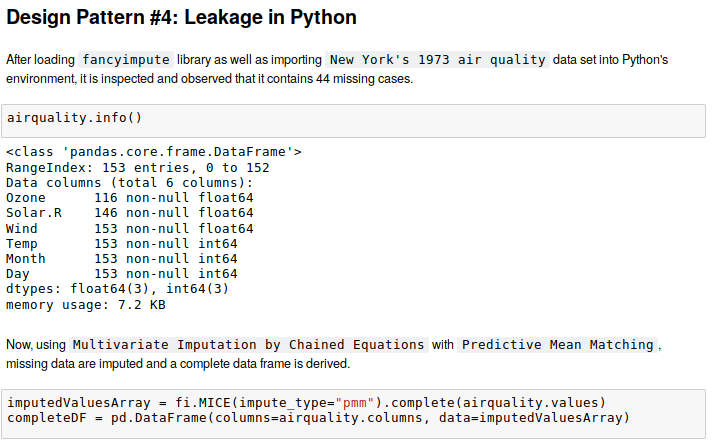
\includegraphics[width=\textwidth+2cm,height=\textheight,keepaspectratio]{images_dp/code_listing_4_leakage}
\caption[Example for Leakage Design Pattern.]{An example for \patternName{Leakage Design Pattern} shows how missing data can be imputed using Python's \mintinline{python}/fancyimpute/ package.
The source code for this pattern is located in \path{code_data/Py_masterThesis.ipynb} file, \path{code_data/R_masterThesis.Rmd} respectively.}
\label{lst:code_pattern4Leak}
\end{figure}

%%%%%%%%%%%%%%%%%%%
\section{Pattern 5: Prototyping}
\paragraph*{Context}
Executives have described in accordance with specific, measurable, assignable, realistic and time-related (SMART) criteria multiple deliverables that they want to receive with a goal of addressing their clients in a better way, and therefore increasing their value to the company.
Such mapping of a business problem to \ac{DS} tasks might include data acquisition and mainly classifying clients into different segments, based on the past transactions predicting sales for the next month and developing simple association rules which might recommend them purchasing new products.

\paragraph*{Problem}
After understanding the nature of data through the exploratory analysis, their transformation, cleaning and potentially imputing missing values, clients need to be classified, sales be predicted and recommendations have to be provided.
Therefore, data scientists need to experiment with simple and complex algorithms that permit them to gain useful insights.

\paragraph*{Forces}
\begin{compactitem}
  \item Having a decisive impact on answering business relevant questions, a variety of statistical models and families exist from which professionals have to identify the right ones and evaluate their performance in line with stated intentions as they all differ in the purpose, interpretability, complexity and accuracy \parencite{SAS2016}.
  \item Furthermore, numerous \ac{ML} applications have become influential as they are flexible for diverse sets of data, easily extensible accommodating new models and metrics and permitting to store intermediate modelling results as well -- all leading to lowering the \ac{DS} bar \parencites{GoebelMichGru1999}{ChenMinMao2014}{EslamiAli2012}.
\end{compactitem}

\paragraph*{Solution}
\ac{KDD} professionals have to identify comprehensive and modular \acp{API} that offer appropriate algorithms for developing \ac{ML} \emph{prototypes}. 
Subsequently, these shall be evaluated to understand how the predictive models perform on unseen data in the future.

When collected information is labelled through attributes, (semi-)supervised learning methods such as \acp{SVM} or naive Bayes are used for predicting the output from input data. 
Depending on different learners and the analytical problem dealt with, two groups of supervised tasks are distinguished -- a \emph{classification} where a target variable is a discrete category or a \emph{regression} where a prediction is a continues numerical value.
On the other hand, when data are unlabelled with no response variable $Y$, more exploratory, unsupervised learning algorithms like $k$-means clustering or principal component analysis are employed to establish groups of similar objects or reduce dimensionality of data \parencites{SAS2016}{NinaBookR2014}.

Continuing with supervised learning, using a \emph{holdout} approach, entire data are at first divided into training (typically about 75\%) and testing set (remaining 25\%; \cite{Kohavi:1995:SCB:1643031.1643047}).
Then, chosen algorithms together with training data are applied for model building. 
Because evaluating prototype's performance on the same data does not tell how well it generalizes, a model is taken with a holdout set to predict outputs and compare its forecast's capability with true data \parencites{FosterProvost2013DataThinking}{JakeVanderPlas2016PythonHandbook}.

\paragraph*{Consequences} ~\\
{\hspace*{14.5pt} \textbf{Benefits:} \hspace*{-5pt} }
\ac{ML} is applicable to diverse industries and use cases and when appropriately applied, a wisdom can be gained which helps decision makers to set right company's objectives and improve products and services to better serve their customers.
Additionally, reflecting the goals, a variety of prototyping metrics can be used for assessing final prediction. 
For example, for classification a confusion matrix is used which \qcite{summarizes the (\dots) predictions against the actual known} classes \parencite[94]{NinaBookR2014}.

\textbf{Liability:}
When complex models are applied, there is a danger of running into a lack of their interpretability \parencite{NadaML2004}. 
Hence, they need to be justified in addition to being regularly updated, verified and improved reflecting changing business operations \parencite{SAS2016}.
Building models may at times also lead to dead paths and accordingly it is necessary to learn quickly from mistakes, and thus maintaining a hub of the past work can support the organization in gaining the knowledge \parencites{Domino2017DS}{SASBP2007}{GoogleDebt1}.
Insufficient quality and quantity of data has a significant impact on the model's predictive power too and for that reason data scientists have to constantly iterate on created prototypes and gather better information \parencites{Zinkevitch2016}{CarlShan2015TheScientists}.

\paragraph*{Known Uses}
\begin{compactitem}
  \item In the unsupervised learning, typical tasks include segmenting (clustering) movies according to the user preferences or creating association rules where market basket analysis establishes customers' items that are frequently bought together \parencites{Trevor2017}{ClusteringAnil2010}{Movies2012}{MBAMR2012}. 
  Furthermore, when data have many potentially redundant features, one may benefit from quicker computation by attempting to reduce $d$-dimensions into $m$ principal components that explain most of the variance in the data \parencites{FieldCadyDSBook}{Tillburg2009}.
  \item In the supervised learning, in the case of regression, it has been attempted for example to predict forest's burned area based on the meteorological data \parencite{ForestFires2007}.
  On the other hand, detecting spam emails has been extensively studied by many researchers as a conventional classification problem \parencite{Brylspam2008}.
\end{compactitem}

\paragraph*{Related patterns}
The exposure to the \emph{bias-variance trade-off} has to be addressed as it can make \ac{ML} prototypes not generalizable beyond the training data, see next \patternName{Cross-validation Design Pattern}.
In addition, \ac{ML} libraries and frameworks have support a range of other capabilities such as later described hyperparameter optimization using \patternName{Grid} or leveraging ensemble methods through \patternName{Assemblage Design Pattern}.

\paragraph*{Sample code}
Because of being in the context of a specific task, an illustrative \mintinline{bash}/Pima Indians Diabetes/ dataset is obtained from \textcite{Lichman:2013} to predict whether females of Pima Indian heritage have diabetes, being a binary classification task. 
Consequently, this is used for illustration in the following three patterns as well. 

In the R ecosystem, two prominent packages exist that provide comprehensive tools for building and evaluating models -- \mintinline{R}/caret/ and \mintinline{R}/mlr/. 
For Python, multiple alternatives are available too, most notably well-established \mintinline{python}/scikit-learn/ for general-purpose \ac{ML}. 

\begin{figure}[!ht]
\centering
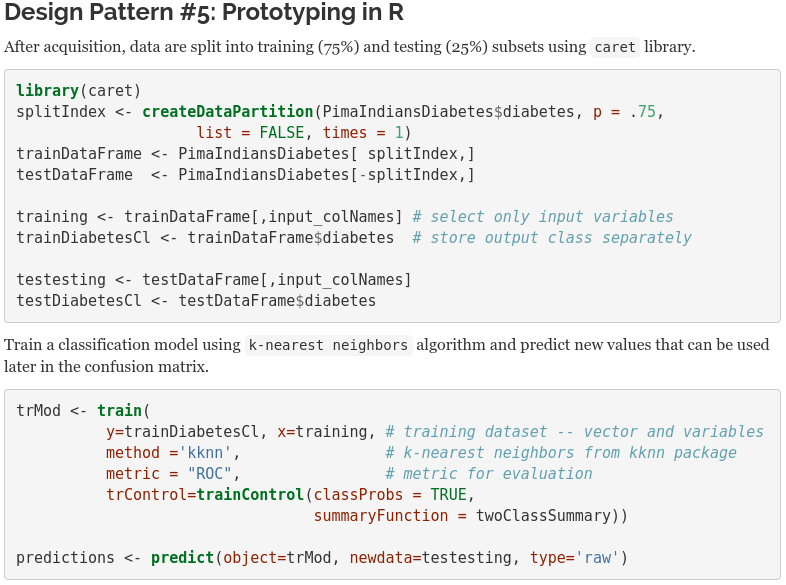
\includegraphics[width=\textwidth+2cm,height=\textheight,keepaspectratio]{images_dp/code_listing_5_prototype}
\caption[Example for Prototyping Design Pattern.]{An example for \patternName{Prototyping Design Pattern} shows R's \mintinline{R}/caret/ library when applied for a classification task using a holdout approach.
The source code for this pattern is located in \path{code_data/R_masterThesis.Rmd} file, \path{code_data/Py_masterThesis.ipynb} respectively.}
\label{lst:code_pattern5}
\end{figure}
%%%%%%%%%%%%%%%%%%%%%%%%%%%%
\section{Pattern 6: Cross-validation}

\paragraph*{Context}
After initial understanding of preferably \emph{tidy} data and the domain being dealt with, a supervised learning algorithm was selected to plausibly satisfy stakeholders' objectives.
Succeeding the \patternName{Prototyping Design Pattern}, the model has to be evaluated as it may not generalize beyond the data which have been used for its creation, causing \emph{overfitting}. 
This means that while originally the learner scored highly on the training data, when previously unseen information arrives, prototype's high complexity leads to a very poor accuracy of a new prediction as it fits noisy data \parencite{NinaBookR2014}.

\paragraph*{Problem}
A major task for any data scientist is to balance the so-called \emph{bias-variance trade-off} where on the one hand \ac{ML} prototype has to account for relevant data features (have high accuracy; in statistical terms low bias) while on the other hand also avoid capturing meaningless data -- that is to have high precision, statistically low variance \parencite{JakeVanderPlas2016PythonHandbook}.
Consequently, one needs to assess learner's predictive power with future data samples using a robust technique which could aid in selecting a model with the lowest bias and lowest variance \parencite{Kohavi:1995:SCB:1643031.1643047}.

\paragraph*{Forces}
\begin{compactitem}
  \item If training and testing prototypes on the same data set, they \enquote{memorize} them very well but this is not representative of the general data trend \parencites{FosterProvost2013DataThinking}{SAS2016}.
  \item Previously, a classical approach tackling overfitting was described where data are randomly split into two sets. 
  This makes a fair approximation by holding back some of the data to validate the prototype with new information.
  However, a portion of valuable data is not training the learner as the test set may be significantly influenced when a random split is not characteristic and balanced \parencites{NinaBookR2014}{FosterProvost2013DataThinking}. 
  \item Although a frequently named alternative is partitioning data into three sets (training, validation and testing), because they are usually small in sample size, a number of examples for \ac{ML} is further reduced. 
  Hence, either holdout approach excludes some information and prevents learning from complete data patterns \parencite{FieldCadyDSBook}.
\end{compactitem}

\paragraph*{Solution}
\emph{Cross-validation} is a sophisticated method for \qcite{generat[ing] multiple performance measures} with an ability to tell what to expect from the forthcoming data by estimating test set (so-called generalization) error \parencite[140]{FosterProvost2013DataThinking}. 
Enhancing the basic holdout technique, it repeats \qcite{the construction of the model on different subsets of the available training data and then evaluate[s it] only on data not seen during construction} \parencite[111]{NinaBookR2014}.

The widely used \emph{k-fold cross validation} splits a data set into $k$, typically five or ten, folds with a goal of training and scoring the prototype $k$ times \parencite{FosterProvost2013DataThinking}.
In each iteration of the cross-validation, $k-1$ different partitions are combined on which the learner is trained and finally its accuracy is estimated on the last fold deriving the overall test performance. 
Having multiple results, these are united by mean for checking the bias and standard deviation for the variance \parencite{NinaBookR2014}.

\paragraph*{Consequences} ~\\
{\hspace*{14.5pt} \textbf{Benefits:} \hspace*{-5pt} }
Compared to the holdout technique described in the \patternName{Prototyping Design Pattern} or \emph{bootstrapping} outlined next, each sample created from cross-validation is certainly used for training and testing step, resulting into reducing the bias as the number of $k$ parts increases \parencite{Gutierrez-Osuna2002LECTURECross-validation}.
Even though it has been sometimes argued that when cross-validation is repeated multiple times, model's variance decreases too, some researchers have not been able to confirm this hypothesis \parencites{Vanwinckelen2012OnCross-validation}{Kohavi:1995:SCB:1643031.1643047}. 

\textbf{Liability:}
Cross-validation is computationally (very) expensive as training and testing steps are rerun $k$ times, specifically with a variation called \emph{leave-one-out cross validation}. 
Despite $k=n$ number of examples, results can still exhibit high variance as well \parencite{Gutierrez-Osuna2002LECTURECross-validation}.

\paragraph*{Known Uses}
\begin{compactitem}
  \item When new data cannot be acquired, cross-validation often becomes \emph{the} method for model building and selection in \ac{DS} through its universality and simplicity \parencites{arlot2010}{CVStandart2008}.
  \item Besides \emph{k-fold cross validation}, variations such as \emph{stratified} or \emph{repeatable cross-validation} have been proposed as well.
  Whereas the objective of the former one is to address biased classes, thus balancing the distribution across each fold making it a good representative of the whole sample, the goal of the latter one is to repeat cross-validation $n$ times creating random data folds whereby subsequent predictions can all be averaged \parencites{KuhnMax2013}{Vanwinckelen2012OnCross-validation}. 
\end{compactitem}

\paragraph*{Related patterns}
As seen next, \emph{cross-validation} is frequently used with the \patternName{Grid} and \patternName{Assemblage Design Pattern}, particularly with the latter one which has the capability of further reducing the overfitting \parencite{NinaBookR2014}. 

An alternative method to cross-validation represents \emph{bootstrapping} which is mainly used for obtaining confidence intervals and where a random sample with replacement of the same size as the original data set is taken for the training step. 
Then, the model is trained on each of them and before results are again averaged, it is also tested on the remaining \qcite{examples that were not selected for training} \parencites{Kohavi:1995:SCB:1643031.1643047}{BookCV201}{Gutierrez-Osuna2002LECTURECross-validation}.  

\paragraph*{Sample code}
Using previously identified R's \mintinline{r}/caret/ and Python's \mintinline{python}/scikit-learn/, a naive Bayes model is demonstrated next where it is applied to four data parts and tested on the fifth one, see Figure \ref{lst:code_pattern7}. 

\begin{figure}[h]
\centering
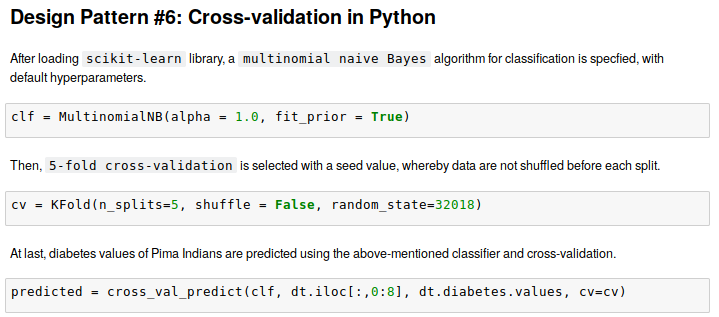
\includegraphics[width=\textwidth,height=\textheight,keepaspectratio]{images_dp/code_listing_6_cv}
\caption[Example for Cross-validation Design Pattern.]{The example for \patternName{Cross-validation Design Pattern} shows application of \mintinline{python}/scikit-learn/ whereby data are first split using five-fold cross validation to which a \emph{multinomial naive Bayes} classifier is applied. 
The complete source code for this pattern is located in \path{code_data/Py_masterThesis.ipynb}, \path{code_data/R_masterThesis.Rmd} respectively.}
\label{lst:code_pattern7}
\end{figure}

%%%%%%%%%%%%%%%%%%%%%%%%%%%%%%
\section{Pattern 7: Grid}

\paragraph*{Context}
\emph{Hyperparameters} are specified in the model before a training step can begin.
While some algorithms have none and can be immediately used for a particular task, others like $k$-means clustering or random forest contain several that data scientists are required to set. 
Typically, in the latter case, one has to decide on a number of trees to build before averaging their predictions \parencite{DL2016Mit}. 
Overall, the importance of hyperparameters lies in having a significant influence on various costs of running the prototype as well as on its behaviour and final performance as seen for instance from \patternName{Prototyping Design Pattern}.

\paragraph*{Problem}
Instead of making (non-)educated guesses to find best hyperparameters by trial-and-error, it is desirable to have an automatic procedure that optimizes them and therefore can increase model's predictive power, its robustness and ultimately generalizability when facing new data.

\paragraph*{Forces}
\begin{compactitem}
  \item Albeit most frequently applied, searching manually for hyperparameters is very time-consuming effort because of their number and having necessary understanding of what they do and what impact they have on the learner \parencite{DL2016Mit}. 
  \item Moreover, retraining each time the prototype because of manually adjusting a large set of hyperparameters can probably lead to omitting some better values.
\end{compactitem}

\paragraph*{Solution}
While designing \ac{DS} pipeline, professionals should employ \emph{grid search} which identifies hyperparameters that deliver best predictions. 
At first, a finite set of values for each hyperparameter is specified in a \emph{grid} which can be in a matrix form through employing \patternName{Data Frame Design Pattern}, simplified for instance \mintinline{bash}/{'k':[2, 4, 6/, \dots, $j$\mintinline{bash}/]}/ and \mintinline{bash}/{'size':[10, 100, 1000/, \dots, $i$\mintinline{bash}/]}/.
Subsequently, the \emph{grid search} algorithm takes the Cartesian product of previous sets $(i_{1...n} \times j_{1...n})$ with $n \in \mathbb{N}_{>0}$ and uses all combinations for training the model \parencite{JakeVanderPlas2016PythonHandbook}. 
After evaluating its performance, typically, by means of \patternName{Cross-validation Design Pattern}, the outcome of such comprehensive search allows to find best settings that should be utilized \parencite{DL2016Mit}.

\paragraph*{Consequences} ~\\
{\hspace*{14.5pt} \textbf{Benefits:} \hspace*{-5pt} }
Even though not guaranteed, choosing a right set of hyperparameters can boost learner's predictive strength by easily parallelizing the computation across a cluster of machines \parencite{BreckMLTest2016}.
Due to being a fairly general approach, one can optimize not only hyperparameters themselves but also finding out the most excellently performing \ac{ML} prototype as well.

\textbf{Liability:}
Searching for best hyperparameters is very \ac{CPU} intensive operation that increases modelling expenses exponentially, particularly when their number to fix is large.
Besides being of $\mathcal{O}(n^c)$ time complexity with $c$ hyperparameters and $n$ number of their values, determining the optimal \emph{grid} to search in may be a task for itself, thus the reliance on experience and third-party resources where similar data or methods were applied \parencite{DL2016Mit}. 

\paragraph*{Known Uses}
Hyperparameter optimization may still lead to overfitting and therefore one ought to combine it with \patternName{Cross-validation Design Pattern} \parencites{JakeVanderPlas2016PythonHandbook}{minleegrid2005}. 
In order to ensure forecast's high-quality, data are at first divided into the training and testing part.
Then, cross-validation splits the training set into $k$-folds. 
For each Cartesian product from the \emph{grid}, a model is trained $k-1$ times and tested on the subset that was left out, leading to record the highest average performance for a particular instance with specific settings.
At last, the one with the best results would be selected for the final step of testing the data from their first separation \parencite{Olson2008}.

\paragraph*{Related Pattern}
Besides aforementioned \emph{grid} and \emph{manual search}, scientists such as \textcites{ReviewHyperOpt2015}{SAS2016} have described other techniques of tuning hyperparameters that have shown to be more convenient and efficient too. 
One of the alternatives presented by \textcite{Bergstra2012RandomOptimization} is named \emph{random search} which takes an arbitrary sample of specified parameters from the \emph{grid} space using a probability distribution like Bernoulli. 
This has proved to achieve very similar results compared to the exhaustive \emph{grid search} but much faster.

\paragraph*{Sample code}
Generally, the majority of comprehensive \ac{ML} packages like those from \patternName{Prototyping Design Pattern} already offer functionality for hyperparameter optimization, including \emph{grid} and \emph{random search}.
Previously used applications \mintinline{r}/caret/ and \mintinline{python}/scikit-learn/ are examples of it.
Consequently, in Figure \ref{lst:code_pattern8}, \mintinline{r}/caret/ package trains a naive Bayes model five times and evaluates it by applying a \patternName{Cross-validation Design Pattern}.

\begin{figure}[h]
\centering
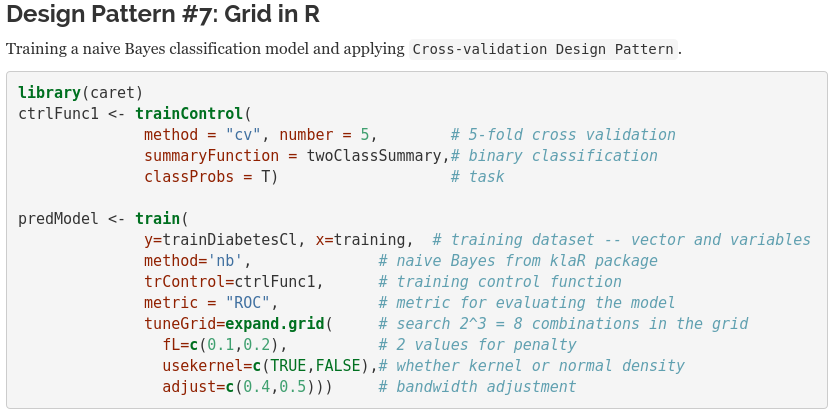
\includegraphics[width=\textwidth,height=\textheight,keepaspectratio]{images_dp/code_listing_7_grid}
\caption[Example for Grid Design Pattern.]{The example for \patternName{Grid Design Pattern} show how naive Bayes model can be trained with \mintinline{r}/caret/ library. 
More specifically, searching the grid with eight hyperparameters and applying five-fold cross-validation.
The complete source code for this pattern is located in \path{code_data/R_masterThesis.Rmd}, \path{code_data/Py_masterThesis.ipynb} respectively.}
\label{lst:code_pattern8}
\end{figure}

%%%%%%%%%%%%%%%%%%%%%%%%%%%%%%
\section{Pattern 8: Assemblage}

\paragraph*{Context}
In the \patternName{Prototyping Design Pattern} it was noted that multiple different algorithms could be used for unsupervised and supervised learning. 
Particularly in the latter case, after training a baseline model and even optimizing its hyperparameters, data scientists ought to judge its performance not only by distinct metrics but also see it in the context of other prototypes to better understand how they behave and compare to each other.
All that in line with \ac{DS} premise of being an iterative process where several alternatives should be build and evaluated.

\paragraph*{Problem}
To further improve achieved results, besides increasing volume of data and their quality through extensive pre-processing, applying for instance \patternName{Leakage Design Pattern} and engineering new features, data scientists may need to intelligently combine outcomes of many diverse models for gaining a greater predictive accuracy in contrast to individual methods alone. 

\paragraph*{Forces}
\begin{compactitem}
  \item A multitude of tested estimators display only mediocre conclusions that are just slightly above a random guess. 
  \item Moreover, even though cross-validation and grid search were administered, it is still possible to observe overfitting that hinders model's practical use for business purposes.
  \item The developed \ac{ML} prototypes carry a large variance due to randomness in hyperparameters, probabilistic nature and selection of data \parencite{NinaBookR2014}.
\end{compactitem}

\paragraph*{Solution}
In the quest of designing high-quality model which is capable of \qcite{reduc[ing] the effect of (\dots) overfitting}, engineers may leverage the power of so-called \emph{ensemble methods} \parencite[426]{JakeVanderPlas2016PythonHandbook}.
These integrate a collection of modelling instances from families such \ac{SVM} or naive Bayes that are diverse and likewise perform differently on the same data \parencite{NagiSajid2013}.
Consequently, their \emph{assemblage} shall lead to improved outcomes and especially \emph{stacking} has been a prominent method. 
This leverages an independent and simple meta-model that combines other prototypes where at first they are individually trained in order to acquire not only their original features but predicted outputs too. 
Then, in the final step of meta learning, the base-level classifiers are basically \enquote{blended} by the super learner algorithm to possibly derive better results \parencites{EnsembleML2012}{Opitz1999}.

\paragraph*{Consequences} ~\\
{\hspace*{14.5pt} \textbf{Benefits:} \hspace*{-5.5pt} }
\emph{Assemblage} of methods attempts to address an instrumental trade-off in \ac{DS}, namely reducing both high variance while at the same time high bias as well \parencite{JakeVanderPlas2016PythonHandbook}. 
Indeed, the accumulation of prototypes has shown to potentially improve final accuracy of prediction by lowering generalization error on unseen data, notably when they contain high amount of variables along with being small in the sample size \parencites{NinaBookR2014}{EnsambleBioinf2010}.

\textbf{Liability:}
Being frequently applied with the \patternName{Grid} and \patternName{Cross-validation Design Pattern}, all three add to the required computing resources \parencite{EnsembleML2012}. 
Primarily, however, \emph{assemblage} further hampers conclusion's interpretability and understandability by the managers creating an undesirable black-box \parencite{PeterETHZ2012}.
Furthermore, if predictions are strongly correlated, one will not be able to boost them with the \emph{ensemble} \parencite{FosterProvost2013DataThinking}. 

\paragraph*{Known Uses}
\begin{compactitem}
  \item Due to universally claiming to improve returns on data of various quality and quantity, practical applications include winning \ac{DS} competitions like Netflix Prize in 2009 where \emph{Gradient Boosted Decision Trees} were applied on hundreds of individual learners to improve company's recommendation engine, see \textcite{Netflix2009}.
  \item \textcites{GranaMichal2014}{NagiSajid2013} have described other use cases such as improved detection of cyber-attacks, prevention of financial fraud, avoiding credit risk or in the medicine for diagnosis of diseases.
\end{compactitem}

\paragraph*{Related Pattern}
Although \emph{stacking} is one of the more advanced \emph{assemblage} techniques, other approaches exist as well \parencite{SAS2016}. 

Considering random forests, these aggregate results from decision trees that are build using training subsets of data sampled with replacement and only with random features \parencite{NinaBookR2014}.
By decreasing the variance, trees can be averaged in parallel to derive the best estimator -- the procedure of which is called \emph{bagging} \parencites{Opitz1999}{PeterETHZ2012}. 

In contrast, \emph{boosting} algorithms like AdaBoost reduce the bias and variance by incrementally building in sequence several \enquote{weak} models that are often only barely better than a random guess \parencite{EnsambleBioinf2010}. 
Aiming to build a combined \enquote{strong} classifier, the idea is to learn from misclassifications of a model instance which culminates into reweighting training data at each round to emphasize shortcomings that should be addressed with a new iteration \parencite{EnsembleML2012}.
Though, not being a silver bullet, overfitting can still occur with outliers and other noise in the data \parencite{BauerErikChan1999}.

\paragraph*{Sample code}
For R, one can use an extension to the previously mentioned \mintinline{R}/caret/ library called \mintinline{R}/caretEnsemble/ or among others \mintinline{R}/SuperLearner/ package. 
Contrarily, besides already shown Python's \mintinline{python}/scikit-learn/ that can be supplemented with \mintinline{python}/Mlxtend/, the example in Figure \ref{lst:code_pattern9} creates an ensemble of two methods using \mintinline{python}/ml-ensemble/ utility. 

\begin{figure}[h]
\centering
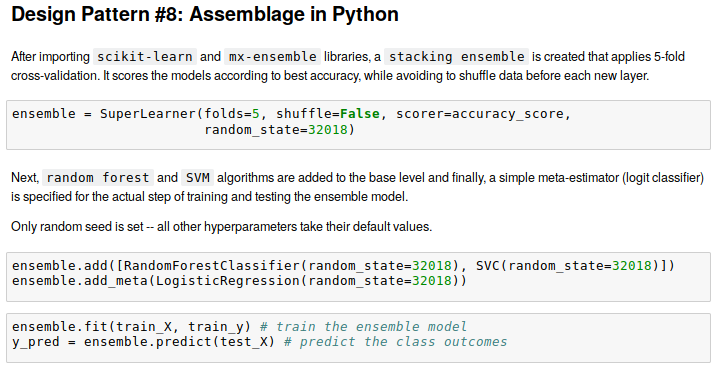
\includegraphics[width=\textwidth,height=\textheight,keepaspectratio]{images_dp/code_listing_8_ensam}
\caption[Example for Assemblage Design Pattern.]{The example for \patternName{Assemblage Design Pattern} displays how a \emph{stacking (logit classifier) ensemble} is constructed to use features from training data through \ac{SVM} and random forest in its resulting prediction.
The complete source code for this pattern is located in \path{code_data/Py_masterThesis.ipynb}, \path{code_data/R_masterThesis.Rmd} respectively.}
\label{lst:code_pattern9}
\end{figure}

%%%%%%%%%%%%%%%%%%%%%%%%%%%%%%
\section{Pattern 9: Interactive Application}

\paragraph*{Context}
After acquiring information about business activities and having answers to questions asked, being one of the concluding steps is when findings are visually communicated in an effective and understandable manner to stakeholders. 
This is done in order to add value to offered services and products and deliver return on \ac{DS} investment.

\paragraph*{Problem}
While the diversity of employee's background and roles manifests in seeking different perspectives to the same underlying data, this is not aligned with conventional reports and presentations which usually display static visualizations and are limited by their scope and a particular view presented -- hence the need for a better alternative.

\paragraph*{Forces}
\begin{compactitem}
  \item Referencing big data properties, information changes rapidly and therefore static graphics may not be relevant in one-week time and so the conclusions based on them. 
  \item Storytelling requires to visualize not only latest data but also enable audience to answer their questions by themselves through adjusting the way information is conveyed in an interactive fashion, for example by drilling it down, without unnecessary latency \parencite{TabPatriVisual2015}.
  \item Business managers are usually not interested in pure numbers without a context and explanation, and thus interpretable results told through diverse means that can easily translate into a set of operational processes and actions are indispensable \parencite{FosterProvost2013DataThinking}.
\end{compactitem} 

\paragraph*{Solution}
As an important part of the communication strategy, data scientists shall design and develop simple, web-based \emph{interactive applications} using the identical programming language applied for other \ac{DS} tasks to stay within the same workflow and avoid technological fragmentation.
Indeed, such applications have to permit users to dynamically interact with presented tables or charts and customize them for their data journey by modifying various graphical and data attributes that reflect employees' own preferences, for instance filtering, zooming or changing the shapes \parencite{WardInteractiveApps2010}. 

\paragraph*{Consequences} ~\\
{\hspace*{14.5pt} \textbf{Benefits:} \hspace*{-5.5pt} }
Stakeholders are provided with a self-service tool that empowers further data exploration, gaining deeper insights by looking at information tooltips and understanding the story through animations and slideshows. 
The information being updated in close to real time makes visualizations display latest available data and consequently fostering a trust and a deeper integration in the organization by allowing to proactively react to the changing environment \parencites{Domino2017DS}{FieldCadyDSBook}.

\textbf{Liability:}
Developing high-quality \emph{interactive application} carries an additional effort in its continuous maintenance due to ever evolving data sources, their granularity and employee desires \parencites{Clarke2013}{Fern2016}. 
Furthermore, it is necessary to understand the targeted technology platform and learn tools for its development.
Besides, when the application has been improperly designed displaying excessive details, technical jargon or having a misguides choice of colours, it ultimately contributes to information overload and never being looked at \parencites{InformaVisualiz}{Gershon1998}{Carr1999}{TabPatriVisual2015}. 

\paragraph*{Known Uses}
\begin{compactitem}
  \item \textcites{DickInteractive2014}{SegelHeer2010} have indicated that interactive stories may possibly enhance a reading experience of a journalistic work on the web.
  \item As already mentioned in the \patternName{Notebook Design Pattern}, dynamic visualizations can be embedded in the document making data analysis more visual from the beginning.
  \item \ac{BI} portals, following best practises in the \ac{UI/UX} design, make available a standard set of core components like sliders for creating \ac{KPI} dashboards with interactive plots.
\end{compactitem}

\paragraph*{Related patterns}
Besides having \emph{interactive applications} on-premise, organizations can take advantage of \emph{cloud computing} services run by providers like Microsoft (\emph{Azure}) or Amazon (\emph{Web Services}). 
This in order to leverage features such as automatic scaling that ensures their uninterrupted availability, see next \patternName{Cloud Design Pattern}. 

\paragraph*{Sample code}
While \mintinline{R}/Shiny/ is almost certainly the most widely used package for developing analytical and interactive web application using R, for Python besides \mintinline{python}/Bokeh/ one can create them by utilizing \mintinline{python}/Plot.ly Dash/ framework too, see Figure \ref{lst:code_pattern10}.

\begin{figure}[ht]
\centering
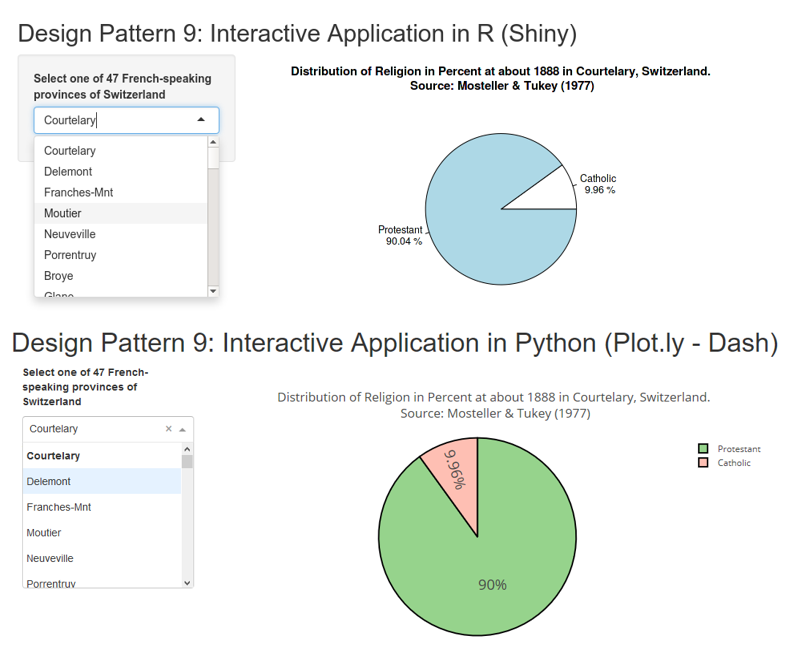
\includegraphics[width=\textwidth,height=\textheight,keepaspectratio]{images_dp/code_listing_9_intApp}
\caption[Example for Interactive Application Design Pattern.]{The example for \patternName{Interactive Application Design Pattern} shows exceptionally a result of R and Python source code located in \path{code_data/dp_9} folder. 
A simple pie chart with a dropdown component where users can choose from a list of provinces is displayed. 
This shows a distribution of religion in Switzerland based on the \emph{Swiss Fertility and Socioeconomic Indicators (1888)} data, obtained through R's \mintinline{R}/datasets/ library.
Upon changing the region (the user interaction), the chart is immediately redrawn to reflect new values.}
\label{lst:code_pattern10}
\end{figure}

%%%%%%%%%%%%%%%%%%%%%%%%%%%%%%
\section{Pattern 10: Cloud}

\paragraph*{Context}
After making available on a local machine a proof of concept which is subsequently validated first by peers in the \ac{DS} team and later by directly involved customers themselves, it is necessary to share the solution with all stakeholders of the organization by deploying it on the production system.

\paragraph*{Problem}
Data scientists need to utilize computing resources in a flexible and simple matter without being constrained by the available hardware and software at company's premises.
The objective of this is to allow for instance quickly scaling up and down \ac{DS} interactive applications or integrating complex predictive models into firm's products and services.

\paragraph*{Forces}
\begin{compactitem}
  \item Organization's core mission is often unrelated to administrating and configuring hardware and software infrastructure. 
  To avoid facing various constrains and difficulties, it has been claimed of being beneficial to outsource the management of servers to experienced specialists \parencite{MarstonSean2011}.
  \item Training \ac{ML} models as well as pre-processing (big) data requires significant computing resources which might impede fast prototyping of \ac{DS} solutions because of the unavailability of modern, on-premise \acp{CPU}, high-volume storage systems and \ac{RAM} in the necessary quantity. 
\end{compactitem}

\paragraph*{Solution}
Instead of building and maintaining own infrastructure, companies and data scientists should learn to utilize \emph{cloud computing} made available by vendors like Google (\emph{Cloud}) or Microsoft (\emph{Azure}). 
While many different types of \emph{cloud} services exist, see \textcite{Zhang2010CloudChallenges} for their overview, a core underlying feature is the ability of on-demand allocation of computing resources paid according to the pay-as-you-go pricing model.  
As such, the \ac{IT} architecture including \ac{DS} workflow shall be designed around leveraging \emph{cloud} features where dedicated data mining virtual machines or enhanced applications for information storage and processing based on the \emph{Hadoop} toolbox might be employed.

\paragraph*{Consequences} ~\\
{\hspace*{14.5pt} \textbf{Benefits:} \hspace*{-5.5pt} }
Perhaps the most important gain is avoiding managing on-premise infrastructure where instead a \emph{cloud} portal permits a rapid provisioning of resources as they are deemed necessary by engineers.
Additionally, it allows to scale organization's \ac{IT} architecture organically and due to using a comprehensive platform which integrates with other offered functionalities, data scientists can focus on understanding the data by taking advantage of a full set of related services \parencites{DJ2013}{Fern2016}.

\textbf{Liability}:
Besides potentially expensive and hence necessity of monitoring used resources, selecting one provider can result into a vendor lock-in because of unique features that may not exist at competitors (or work in a similar matter; \cite{JusticeMartinis2015Cloud}). 
Moreover, security and privacy concerns can put \emph{cloud computing} either in jeopardy or substantially increase technological and bureaucratic burdens due to legal compliance and regulations \parencite{StoneAdamPrivSecCloud2010}.
Furthermore, companies may not be culturally and process-wise ready to take its advantages by reasons of lacking in-house expertise.

\paragraph*{Known Uses}
\begin{compactitem}
  \item Typically, the power of \emph{cloud} complements natural language processing or object recognition in images and at the same time enables quicker training of predictive models and management of the whole \ac{DS} workflow and \ac{ETL} pipeline.
  \item Likewise, third-party \emph{cloud} services can reinforce good software engineering practises such as continuous integration and platform agnostic development and deployment \parencite{GuhaSEngCloud2010}. 
  \item \ac{KDD} newcomers without programming skills may use various \emph{\ac{ML} Studios} -- cloud-based web applications, often in conjunction with \patternName{Notebook Design Pattern} -- that offer a simple drag-and-drop functionality for building a visual pipeline that contains operations for importing data sources, their processing, model building and visualization.
\end{compactitem}

\paragraph*{Related Patterns}
As previously mentioned, \emph{cloud computing} is applicable at many stages of \ac{KDD} process -- when both developing \ac{DS} solutions including \ac{ML} prototypes and interactive applications as well as during their subsequent final deployment.

\paragraph*{Sample code}
In the past decade, due to a variety of established \emph{cloud(-enhanced)} solutions by numerous providers, see \textcites{Durao2014AComputing}{Zhang2010CloudChallenges}, the availability of R and Python packages that connect to these services is depending on vendors to provide them and the community interest to develop them. 

Some examples include R' \mintinline{R}/cloudml/ package that interacts with specific \acp{API} offered by Google's \emph{Cloud Machine Learning Engine}.  
Alternatively, \mintinline{R}/doAzureParallel/ library supports parallel execution on Microsoft's \emph{Azure} virtual machines.
Similarly, several software development kits for Python exist as well. 
One of them is Amazon \emph{Web Services'} \mintinline{Python}/Boto3/ package that encompasses numerous \acp{API} which can access \ac{ML} capabilities including what the company calls \emph{vision} or \emph{language services}.

For the simplicity of the illustration, previous examples from the \patternName{Interactive Application Design Pattern} can be deployed to two \emph{platform-as-a-service (PaaS) cloud computing} environments.
These provide a complete \qcite{platform (\dots), including operating system support and software development frameworks} for the management of applications while at the same time giving no control over the infrastructure itself \parencites[10]{Zhang2010CloudChallenges}{Pahl2015ContainerizationCloud}. 
Consequently, \mintinline{python}/Plot.ly Dash/ example is served by \mintinline{bash}/Heroku.com/\footnote{\href{https://designpattern10.herokuapp.com/}{https://designpattern10.herokuapp.com/}}, whereas R's alternative using \mintinline{R}/Shiny/ framework could be pushed to \mintinline{bash}/shinyapps.io/, see Listing \ref{lst:code_pattern11}. 

\begin{listing}[H]
  \begin{minted}[breaklines, linenos]{R}
> library(rsconnect) # loads the package for shinyapps.io

# set up the user account with complete API keys, omitted for brevity
> setAccountInfo(name='dmpe',
        token='820739C8B8B9DE...',
        secret='gAHFGNCdDlUtzo...') 

# once deployed, navigate the browser to it
> deployApp(appDir = "/code_data/dp_9/R-Shiny", 
          appName = "DesignPattern10-InteractiveApplicationOnCloud", 
          launch.browser = TRUE)
  \end{minted}
\caption[Example for Cloud Design Pattern.]{The example for \patternName{Cloud Design Pattern} displays how \mintinline{R}/Shiny/ application can be deployed to a third-party PaaS hosting to leverage integrated features like automatic scaling and advanced monitoring.
The source code for this pattern is located in \path{code_data/dp_10} folder.}
\label{lst:code_pattern11}
\end{listing}

%%%%%% 			DSTM
\section{Data Science R and Python Toolkit Matrix}
As explained in the \textbf{chapter \ref{chap:Method}} and seen previously, during pattern discovery and description, R and Python code examples were provided for each pattern candidate, see likewise \path{code_data} folder in the supplement.  
Indeed, thirty-two R and Python packages were identified having followed outlined criteria mentioned in Table \ref{tab:creteriaIncExcl} and subsequently they were recorded in the database shown in Figure \ref{fig11}. 
In line with the third research question and once all design patterns were refined, libraries were finally visualized in a mind-map in Figure \ref{DTSMmindmapWithout}.
Thus, allowing to enact a foundational perspective on the ecosystems of two languages and their available tools \parencite{SuriHarsh11}.

Moreover and where applicable, an attempt was made to present native approaches which were integrated into the respective programming language. 
Unfortunately, while four cases were identified in R, illustratively \mintinline{R}/reshape()/ function that is related to \patternName{Tidy Data Design Pattern}, for Python none were recognized in its \emph{standard library} that could directly interconnect with one of ten design patterns \parencite{PythonCoreStandartLib}.   

%%%%%%%%%%%%%
\section{Summary}
Attempting to shed light on the second study question, after understanding key terms used in this work and presenting the methodology, \textbf{this chapter} was fundamental as ten data science design patterns candidates were formalized. 

As stated in objectives of this work, it has been furthermore asked what R and Python tools from both ecosystems can be found solving common obstacles arising from the knowledge discovery process and being in relation to identified design patterns. 
By purposefully surveying both landscapes, a sample of thirty-two packages was visualized in the \acl{DSTM} as well.

In the \textbf{final chapter} and not being limited to, these core outcomes are individually discussed. 

\begin{landscape}
\begin{figure}[ht]
\centering
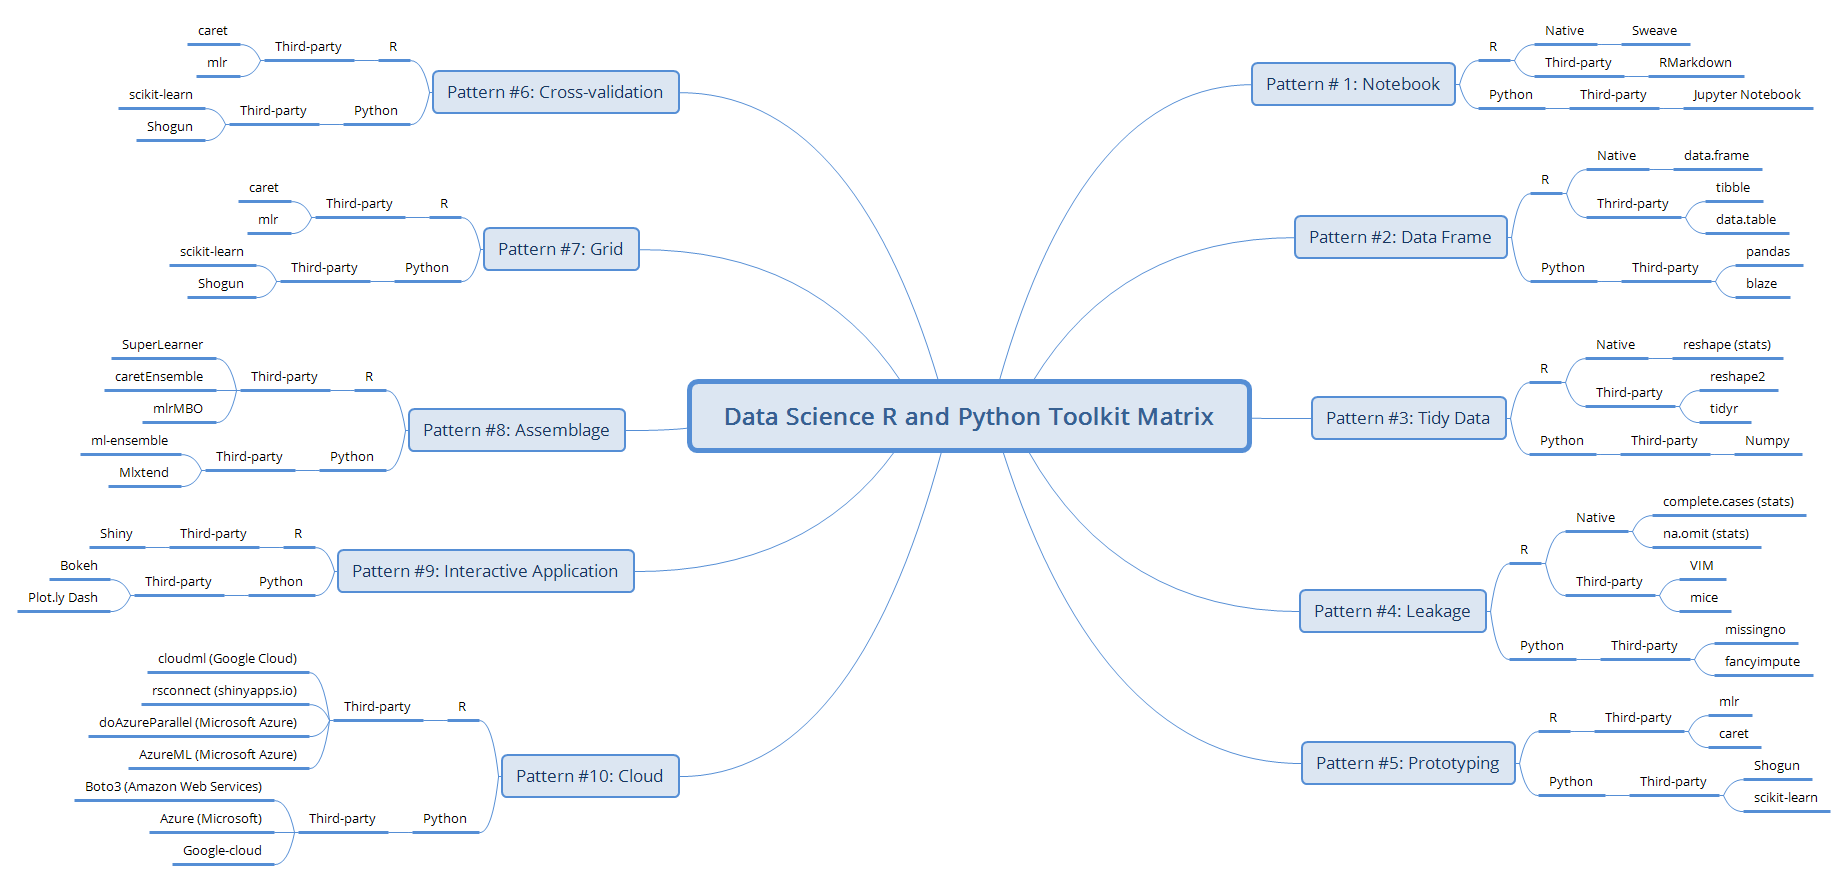
\includegraphics[width=\textwidth,height=\textheight,scale=0.9,keepaspectratio]{images/Data_Science_R_and_Python_Toolkit_Matrix.png}
\caption[Illustrates \acl{DSTM}.]{Illustrates \acl{DSTM} that consists of thirty-two packages and where applicable also with (R) native approaches that were incorporated into the language itself.}
\label{DTSMmindmapWithout}
\end{figure}
\end{landscape}


